% !TeX spellcheck = es_ES 
\documentclass{article}

\usepackage[section]{placeins}
\usepackage{enumerate}
\usepackage{makecell} 
\usepackage{graphicx}
\usepackage{url}
\usepackage[spanish]{babel}
\usepackage[utf8]{inputenc}
\usepackage[backend=biber, style=numeric]{biblatex}
\addbibresource{PROTOCOLO_RSL.bib}

\begin{document}
  \title{%
  Protocolo \\
  \large Revisión de la literatura sobre las actividades de requisitos para Software como Servicio\\}
  \author{Alberto de Jesús Sánchez López \\ 
  \small Proyecto Guiado}
  \date{Fecha}
  \maketitle
  \thispagestyle{empty}
  \newpage

  \tableofcontents
  \thispagestyle{empty}
  \newpage

\setcounter{page}{1}
\section{Introducción}
Desarrollar un producto de \emph{software} que pueda ser distribuido en un modelo de \emph{software} como servicio 
es un proceso complejo, porque el  producto debe aportar un conjunto de ventajas funcionales hacia el usuario final, 
éstas ventajas representan un valor competitivo a empresas de alto impacto interesadas en entrar en un mercado. Es importante 
mencionar que no existen procesos logísticos externos, ya que la gestión del producto se lleva a cabo en su totalidad, en línea.
Lo anterior permite olvidarse de problemas relacionados a la gestión interna de las funcionalidades del software, 
esto se traduce en una forma efectiva de mitigar costos operacionales dentro de la empresa. 

Por lo tanto, la creación de un \emph{software} como servicio representa un conjunto de retos, debido a que las 
metodologías y estrategias tradicionales no cubren las necesidades para desarrollar un \emph{Saas}. lo que hace necesario adecuar el conocimiento 
existente \cite{wanderley2017requirements}. El éxito de un \emph{Saas} depende de entender y definir el conjunto de requisitos dictados por cliente o mercado \cite{4960886}, 
la fase de requisitos, es crucial para delimitar el alcance del proyecto, analizar, documentar y verificar los servicios y restricciones del sistema. 
Una definición de requisitos que ha sido desarrollada siguiendo un conjunto de estrategias formales,  
es de suma importancia para el éxito del proyecto \cite{6530271} ya que esto asegura que la especificación de requisitos ha sido 
realizada siguiendo un proceso y por ende los fundamentos necesarios para el correcto diseño de la solución son confiables
lo que asegura que existe un conocimiento definido de las necesidades del sistema..
Sin embargo no existen metodologías fundamentales relacionadas al desarrollo y gestión de requisitos para un \emph{Saas}, no existe evidencia 
formal que ataque el proceso de elicitación y gestión de cambios de requisitos en el dominio de \emph{Software} como servicio \cite{7037656}. 

Para analizar el estado de las investigaciones actuales sobre el tema se llevaron a cabo búsquedas de estudios secundarios 
relacionados al proceso de requisitos en un \emph{software} como servicio o computación en la nube, se encontraron
dos estudos secundarios de interés.
El estudio secundario \cite{zalazar2017analyzing} identifica las metodologías utilizadas para el proceso de requisitos en sistemas de la nube,
clasifica a los stakeholders considerados en el proceso de requisitos y clasifica las dificultades encontradas en publicaciones 
relacionadas a requisitos para cómputo en la nube, la investigación realiza una identificación y clasificación, de metodologías soportadas, de forma general
el acercamiento hacia los roles es puramente organizacional y no se detallan las actividades típicas realizadas por los roles señalados en el estudio. 
En el segundo estudio secundario \cite{wanderley2017requirements} se realizó un análisis de metodologías, modelos o herramientas para abordar requisitos en sistemas en la nube, el estudio 
señala el enfoque principal de investigaciones, el tipo de distribución utilizada en las publicaciones seleccionadas y las fuentes de distribución de 
estudios primarios relacionados al \emph{software} como servicio. 

Los estudios anteriores, no se encargan de cerrar el vacío de conocimiento en el área de requisitos para un software como servicio, ya que ninguno de los dos 
analiza el estado del arte de las actividades de requisitos para un \emph{software} como servicio. Esto representa una oportunidad para realizar una revisión
sistemática de la literatura, con el objetivo de analizar e identificar las actividades relacionadas a requisitos en un \emph{software} como servicio,
Esto permitirá a investigadores y estudiantes obtener una recopilación reciente del conjunto de estrategias utilizadas para definir los fundamentos de un producto, 
así como ofrecer un conjunto de áreas de investigación abierta.


\newpage

\section{Esquema de Fundamentos}
Como parte del conjunto de investigaciones realizadas en la Facultad de Estadística e Informática, con el propósito de
explorar campos de conocimiento relacionados al \emph{software, platform e infrastructure as a service}, se encuentra 
la monografía realizada por \cite{hernandez2020xaas}, que se encargó de realizar una compilación de los textos  
relacionados al modelo de distribución \emph{XaaS} (por su siglas en inglés, todo como servicio). En el trabajo, se propone
mantener actualizado el estado del arte de los modelos de distribución en crecimiento o tecnologías que posibilitan 
las condiciones necesarias para llevar a cabo emprendimiento de alto impacto. 

En el contexto mundial actual, la pandemia producida por el virus SARS-CoV-2 (COVID-19) ha resultado en el incremento de  adopción de servicios \emph{cloud} y 
productos con modelo \emph{as a service}, en sectores enfocados a educación en línea, cuidado de la salud y \emph{e-commerce} \cite{value:online} .
Esto se ha provocado debido a que existen empresas dipuestas a adquirir tecnología como un medio para reducir costos y ofrecer mejor calidad en los
servicios, con solo rentar el derecho de utilizar un producto o solución de infraestructura \cite{Wu2011}.
Se adopta el servicio, con la justificación de encontrar valor competitivo o mejora del rendimiento en el servicio a prestar \cite{oliveira20191}.
En resumen, un \emph{software} como servicio puede ser representado como un conjunto de necesidades complejas, dinámicas y extensas, 
las cuales se traducen en un conjunto de requisitos que deben ser identificados, clarificados, 
gestionados y documentados, por medio de un proceso formal. 

La gestión de los requisitos se divide en un conjunto de actividades; elicitación, análisis, especificación y validación \cite{abran2004software}
ëstas disciplinas, abarcan las tareas involucradas con explorar, evaluar, documentar y validar los requisitos de un producto. \cite[p.15]{2543993}.








\newpage

\section{Preguntas de investigación}\label{pi}
El objetivo de la Revisión Sistemática de la Literatura es encontrar el estado del arte del las actividades de requisitos para un \emph{software} como servicio. 

\begin{enumerate}[P 1.-]
  \item\emph{¿Qué técnicas de elicitación se han utilizado para la identificación de requisitos de Software como Servicio?}
  \begin{enumerate}[(a)]
  \item \emph{¿Qué técnicas de elicitación se aplican?}
  \item \emph{¿Qué retos se presentan en la elicitación?}
  \end{enumerate}
  Motivación: Señalar el conjunto de técnicas utilizadas para llevar a cabo un proceso de elicitación de requisitos para un software como servicio e identificar los retos encontrados en el proceso de elicitación. 
  
  \item\emph{¿Qué técnicas de análisis se han utilizado para la definición de requisitos de Software como Servicio?}\\
  Motivación: Identificar las actividades realizadas para llevar a cabo el proceso de análisis, clasificación y definición de un conjunto de requisitos para un software como servicio.

  \item\emph{¿Qué actividades se han utilizado para llevar a cabo la validación de los requisitos de un Software como Servicio?}\\
  Motivación: Identificar las técnicas que utilizadas para definir un proceso de validación de requisitos para un software como servicio.

  \item\emph{¿Qué actividades se han utilizado para gestionar los cambios de requisitos de un Software como Servicio?}
  \begin{enumerate}[(a)]
  \item \emph{¿Cómo se evalúan los cambios en los requisitos?}\
  \end{enumerate}
  Motivación: Señalar las actividades utilizadas para gestionar cambios de requisitos en un software como servicio encontradas en la literatura.
            
  \item\emph{¿Qué actividades se han utilizado para gestionar riesgos asociados a los requisitos de un Software como Servicio?}
  \begin{enumerate}[(a)]
  \item \emph{¿Cómo se identifican los riesgos?}
  \item \emph{¿Cómo se controlan los riesgos?}
  \end{enumerate}
  Motivación: Identificar las actividades utilizadas para señalar y controlar los riesgos relacionados a cambios de requisitos en un software como servicio. 
  
  \item\emph{¿Qué temas abiertos se identifican en la literatura reciente en el desarrollo de Software como Servicio?}
  \begin{enumerate}[(a)]
  \item \emph{¿Qué temas abiertos existen relacionados a las actividades llevadas a cabo en la gestión de requisitos de un software como servicio?}
  \end{enumerate}
  Motivación: Identificar los temas abiertos sugeridos en la literatura relacionada a las actividades de elicitación, análisis, validación y gestión de cambios 
 para requisitos de un software como servicio.
\end{enumerate}


\section{Estrategia de búsqueda}\label{Estrategia de búsqueda}

\subsection{Términos de búsqueda}
Los siguientes términos de búsqueda fueron seleccionados con el propósito de identificar los estudios que 
permiten proveer evidencia relevante a las preguntas de investigación definidas. 
Para lograr lo antes mencionado, se llevaron a cabo un conjunto de búsquedas piloto con el fin de encontrar
un conjunto de términos de búsqueda adecuados para hallar investigaciones primarias relevantes a 
la revisión sistemática de la literatura, a continuación se muestran los términos seleccionados.

\begin{table}[ht]
        \caption{Términos de búsqueda} 
        \centering 
        \begin{tabular}{c c}
                \hline
                Concepto & Término de búsqueda\\ [0.5ex] % inserts table
                %heading
                \hline
                Requisitos             & \makecell{Requirements Engineering \\
                                                   Collaborative Requirements} \\
                \hline 
                Software como servicio & \makecell{Software as a Service \\
                                                   SaaS \\
                                                   Cloud Computing }\\ [1ex]
                \hline 
        \end{tabular}
        \label{table:tablaterminos}
\end{table}
\newpage

\subsection{Cadenas de búsqueda}
Basado en la estructura de las preguntas de investigación, se extrajo un conjunto de 
términos de búsqueda, éstos serán utilizados con el objetivo de definir una cadena de búsqueda apropiada para 
las necesidades de la RSL. En el proceso de llevar a cabo búsquedas piloto, se utilizaron los siguientes terminos 
de interés extraídos de las preguntas de la investigación 
\emph{Requirement* y Elicitation o Validation o Analysis o Management o Risk Management}, las búsquedas con estos 
términos resultaron en un grupo de estudios primarios que no eran de importancia para alcanzar el objetivo de la 
revisión sistemática. 

Según lo anterior se estableció la siguiente cadena. 

\emph{(Requirement* Engineering OR Collaborative Engineering AND (Software as a service or Saa* or Cloud computing))}







\subsection{Selección de fuentes}
Seleccionar bases de datos relevantes en el área de Tecnologías de la Información 
e Ingeniería de \emph{Software}, es fundamental para una revisión sistemática 
de la literatura.  Se seleccionaron las fuentes de información desplegadas en el Cuadro \ref{tablafuentes},
ya que disponen de acceso a trabajos sustanciales en los campos de ingeniería de requisitos y software como servicio, 
así como también a las conferencias y journals importantes. 
Antes de definir el conjunto de bases de datos, se llevaron a cabo 
búsquedas prueba, esto culminó en la exclusión  de \emph{Google Schoolar}, 
por el número de artículos repetidos.\\
Es importante notar que cada fuente de datos contiene un conjunto de opciones para búsquedas avanzadas, 
esto se tomó en cuenta para posteriormente, diseñar criterios individuales con el objetivo de mejorar la calidad de inclusión de los 
artículos de interés para el estudio.


\begin{table}[ht]
        \caption{Fuentes seleccionadas\strut}
        \label{tablafuentes} 
        \centering 
        \begin{tabular}{c}
                \hline
                Fuentes \\ 
                %heading
                \hline 
                \makecell{iEEE Explore\\
                          Science Direct\\
                          ACM Digital Library} \\ [1ex] 
                \hline 
        \end{tabular}
\end{table}
\newpage

\section{Selección de estudios primarios}
Se seleccionó búsqueda automatizada con \emph{backwards snowballing} sugerida por \cite{kitchenham2007guidelines} para obtener el mayor número de 
artículos posibles, con un alto nivel de precisión.
Para validar el proceso de selección, se llevarán a cabo un conjunto de búsquedas 
informales en librerías indexadoras, fuentes digitales y conferencias influyentes en el área de 
servicios cloud, también búsquedas manuales para validar que los estudios base sean encontrados utilizando
el proceso de búsqueda, las fuentes, criterios de inclusión y exclusión y síntesis de los datos.

La completetitud de análisis de los estudios primarios se ha definido como importante ya que 
existe un conjunto limitado de estudios. Para mitigar lo anterior, se ha añadido el proceso de 
\emph{backwards snowballing}.
El conocimiento adquirido en los estudios es de alta importancia, ya que las actividades 
internas del proceso de requisitos en un software como servicio puede variar a través de los estudios
seleccionados y es importante analizar un rango amplio de estudios que proyecten el estado actual del arte 
de requisitos de un \emph{software} como servicio. 

\subsection{Criterios de selección de estudios primarios}
Se definieron criterios de inclusión y exclusión con el objetivo 
de seleccionar investigaciones que respondan las preguntas de investigación, con la finalidad de ser  
sintetizadas para extraer su información al fin de la revisión de estudios.
Se incluyen solo estudios primarios escritos en inglés (CI-1) ya que no existe el
recurso humano para traducir estudios en otros idiomas, durante las búsquedas piloto 
se definió incluir estudios realizados entre 2010  y enero del 2021, ya que es importante
encontrar trabajos relevantes recientes relacionados al software como servicio, 
se excluye literatura informal (CE-1), estudios duplicados (CE-2), se incluyen 
estudios según el análisis de título y abstract (CI-3) y (CI-4),
se incluye si el texto completo contesta a alguna de las preguntas de investigación (CI-5), 
se excluye si es una versión previa a un estudio más completo (CE-3), o si no es posible acceder desde la fuente 
de información (CE-4).


\subsection{Criterios de inclusión}
\begin{enumerate}[C-1.-]
  \item{Es un estudio primario escrito en inglés.}
  \item{Es un estudio primario publicado entre 2010 - enero del 2021.}
  \item{El título y el abstract deben contener al menos dos términos de búsqueda.}
  \item{El título y el abstract dan indicios de que se concentrará en una de las preguntas de investigación.}
  \item{El texto completo contesta a alguna de las preguntas de investigación.}
\end{enumerate}

\subsection{Criterios de exclusión}
\begin{enumerate}[CE-1.-]
  \item{Es un libro, capítulo de libro, curso o estándar.}
  \item{Es un estudio primario duplicado. (Aparece en más de una base de datos.)}
  \item{Es una versión previa a un estudio más completo sobre la misma investigación.}
  \item{No se tiene acceso al texto completo.}
\end{enumerate}
\newpage

\subsection{Procedimiento de selección de estudios primarios}
Se definieron las siguientes etapas para la selección de estudios primarios con el fin 
de filtrar de forma eficaz la selección de estudios, para facilitar la selección y análisis 
del conjunto de estudios, con el fin de obtener una base de conocimientos relevantes. 

\subsection{Etapa número uno}
\begin{enumerate}[(a)]
  \item{Idioma inglés. (CI1)}
  \item{Publicado entre 2010-2021. (CI2)}
  \item{No es un libro, capítulo de libro, curso o estándar. (CE1)}
  \item{Contiene al menos dos términos de búsqueda. (CI3)}
\end{enumerate}

\subsection{Etapa número dos}
\begin{enumerate}[(a)]
  \item{El título y abstract dan indicios de que se trata del dominio de interés. (CI4)}
  \item{No duplicados. (CE2)}
  \item{No hay versiones anteriores. (CE3) }
  \item{Acceso al texto completo. (CE4)}
\end{enumerate}

\subsection{Etapa número tres}
\begin{enumerate}[(a)]
  \item{Texto completo contesta alguna pregunta de investigación. (CI5)}
\end{enumerate}
\newpage

\section{Evaluación de calidad}
Incluso si no existe un éstandar que establezca las caracteristicas de un estudio 
de alta calidad, hay un consenso común sobre el impacto de los estudios primarios 
en los resultados de una revisión sistemática de la literatura, por eso y utilizando 
preguntas definidas según \cite{kitchenham2007guidelines} el fin de evaluar de forma correcta en el contexto actual. 

\begin{center}
\begin{table}[ht]
        \caption{Calidad} 
        \centering 
        \scalebox{0.7}{
        \begin{tabular}{c c c}
                \hline
                Criterios & Grado & Grado obtenido\\ [0.5ex]
                %heading
                \hline 
                (C1) ¿Es el objetivo del estudio definido de forma clara? & {1, 0.5, 0} {Si, Nominalmente, No} \\
                \hline
                (C2) ¿El contexto del estudio está bien definido? & {1, 0.5, 0} {Si, Nominalmente, No} \\
                \hline 
                (C3) ¿Los resultados son claros? & {1, 0.5, 0} {Si, Nominalmente, No} \\
                \hline
                (C4) Según los resultados, ¿Que tan valioso es el estudio? \\
                \hline 
        \end{tabular}}
        \label{table:tablacalidad}
\end{table}
\end{center}

\newpage

\section{Extracción de los datos}
El proceso de extracción de los datos se llevará a cabo por el estudiante autor de la RSL, según la guía realizada por
\cite{kitchenham2007guidelines} se recomienda que los supervisores realicen búsquedas prototipo en un conjunto de estudios al azar para evaluar la consistencia
en la extracción de datos.

\subsection{Formato para extracción de los datos}
La siguiente tabla ha sido desarrollada con el propósito específico de extraer datos de interés para la investigación, 
los datos deben estar relacionados a las preguntas de investigación, para poder ser analizados posteriormente 

\begin{center}
\begin{tabular}{ |l|l| }
\hline
\multicolumn{2}{|c|}{Datos generales} \\
  \hline
    Identificador &       \\
    \hline
    Título & \\
    \hline
    Autores &\\
    \hline
    Daño & \\
    \hline
    Fuente & \\
    \hline
    Título de publicación (memorias, \emph{journal}, etc.) & \\
    \hline
    DOI & \\
    \hline
    Palabras clave & \\
    \hline
    \emph{Abstract} o resumen & \\
    \hline
    Pregunta/s de investigación relacionada/s & \\
    \hline
    Técnica/s identificada/s para elicitación& \\
    \hline
    Reto/s identificado/s en el uso de técnicas de elicitación& \\
    \hline
    Técnica/s de análisis de requisitos identificadas& \\
    \hline
    Técnica/s utilizada/s para validar requisitos & \\
    \hline
    Actividade/s identificada/s para llevar a cabo la gestión de requisitos& \\
    \hline
    Actividade/s identificada/s para definir riesgos asociados a requisitos& \\
    \hline
    Tema/s abierto/s propuesto/s en el área de requisitos en el software como servicio& \\
    \hline
 \hline
\end{tabular}
\end{center}

\section{Estrategia para la síntesis de datos}
Según la guía realizada por \cite{kitchenham2007guidelines} se ha decidido utilizar síntesis cualitativa, para identificar y estructurar los resultados compuestos por 
lenguaje natural, resultantes del proceso de búsqueda, empleando el \emph{approach} traducción recíproca sugerido por REFERENCIA con el fin de señalar 
y sintetizar el conjunto de actividades identificadas.
\newpage

\section{Limitaciones}
\subsection{Amenazas a la validez: Internas}
El factor principal a ser considerado como restricción es que el estudio presente está siendo 
desarrollado por un estudiante de licenciatura, para minimizar esta amenaza, que puede afectar a la objetividad 
al realizar la RSL se tomó como referencia la guía realizada por \cite{kitchenham2007guidelines}
como guía para llevar a cabo la RSL, también se definieron evaluaciones de la calidad del trabajo, en conjunto 
con los directores de la revisión para mitigar cualquier amenaza a la objetividad de la investigación. 

\subsection{Amenazas a la validez: Externas}
El campo de software como servicio es nuevo y sigue en crecimiento, esto se hace notorio en la escasez de 
RSL relacionadas al tema, por lo tanto se define lo anterior como  una amenaza externa ya que, un conjunto 
de revisiones sistemáticas podrían formar una base de fundamentos para el desarrollo de temas de investigación, el cual no existe.
\newpage


\section{Informe}
\subsection{Titulo}
\subsection{Resumen}
\subsection{Introducción}
\subsection{Antecedentes}
\subsection{Método}
\subsection{Resultados}
\subsection{Discusión}
\subsection{Conclusión}
\newpage

\section{Gestión de la revisión}

\subsection{Cronograma}
El cronograma muestra las actividades a llevar a cabo en los meses de noviembre a enero.

\begin{figure}[!htb]
    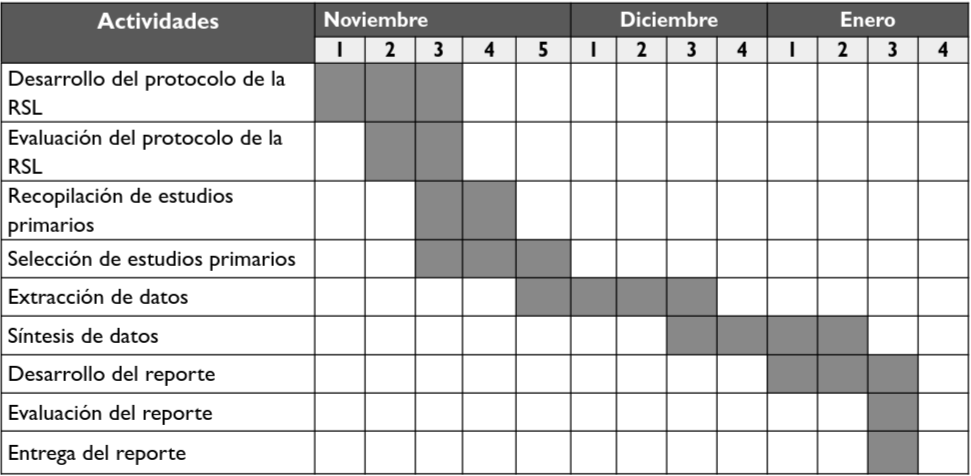
\includegraphics[width=\linewidth]{gant.png}
    \caption{Cronograma de actividades.}
    \label{fig:grant}
\end{figure}

\subsection{Herramientas utilizadas}
Se utilizó LaTex para llevar a cabo el documento del protocolo, para almacenar referencias 
se crearon diferentes archivos, los cuales contienen referencias, todos han sido 
almacenados con extensión .bib, se empleó BibTex para llevar a cabo las referencias a las 
investigaciones o documentos de interés, guardó la hoja de cálculo en la que se llevó 
a cabo búsquedas prueba y se se gestionó el proceso de control del documento con .git,
los archivos de referencias han sido alojados en GitHub,
\newpage

\subsubsection{Paquete de replicación}
Como un aporte a la comunidad de investigación en el área de ingeniería de \emph{software}, 
se añade un paquete de replicación de la investigación, con el objetivo de aportar  
al conjunto de estudiantes e investigadores interesados y de esta forma avanzar y distribuir 
conocimiento.
El paquete de replicación también será una herramienta importante utilizada con el fin de replicar 
el proceso de investigación llevado a cabo.

Lista de items incluídos en el paquete: 
  \begin{enumerate}[(a)]
  \item Anteproyecto con descripción de objetivo y contexto de la investigación. 
  \item Lista de referencias utilizadas como fundamento de conocimiento. (.bib)
  \item Lista de referencias utilizadas en el protocolo.  (.bib)
  \item Protocolo.
  \item Tabla de \emph{Google sheets} con detalle de búsquedas piloto realizadas. 
  \item Lista de referencias utilizadas en el protocolo de investigación.
  \end{enumerate}
\newpage

\section{Referencias}
\printbibliography

\end{document}
